% Title: gl2ps_renderer figure
% Creator: GL2PS 1.4.2, (C) 1999-2020 C. Geuzaine
% For: Octave
% CreationDate: Sat Sep 11 17:34:49 2021
\setlength{\unitlength}{1pt}
\begin{picture}(0,0)
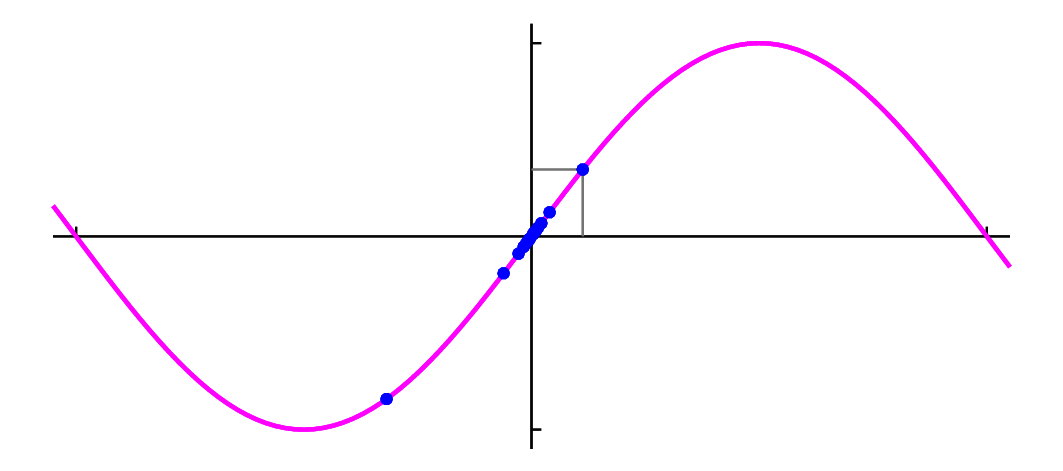
\includegraphics[width=9cm,height=4cm]{fig_teorema_funcao_continua_1}
\end{picture}%
\begin{picture}(255,113)(0,0)
\fontsize{10}{0}\selectfont\put(18.2667,48.8036){\makebox(0,0)[t]{\textcolor[rgb]{0.15,0.15,0.15}{{$-\pi$}}}}
\fontsize{10}{0}\selectfont\put(236.851,48.8036){\makebox(0,0)[t]{\textcolor[rgb]{0.15,0.15,0.15}{{$\pi$}}}}
\fontsize{10}{0}\selectfont\put(122.568,9.92197){\makebox(0,0)[r]{\textcolor[rgb]{0.15,0.15,0.15}{{-1}}}}
\fontsize{10}{0}\selectfont\put(122.568,102.692){\makebox(0,0)[r]{\textcolor[rgb]{0.15,0.15,0.15}{{1}}}}
\fontsize{10}{0}\selectfont\put(120.601,72.3672){\makebox(0,0)[r]{\textcolor[rgb]{0,0,0}{{$b_k=f(a_k)$}}}}
\fontsize{10}{0}\selectfont\put(139.859,51.6686){\makebox(0,0)[tl]{\textcolor[rgb]{0,0,0}{{$a_k$}}}}
\end{picture}
